\documentclass[convert={density=300,outext=.png}]{standalone}
\usepackage{tikz}

\begin{document}
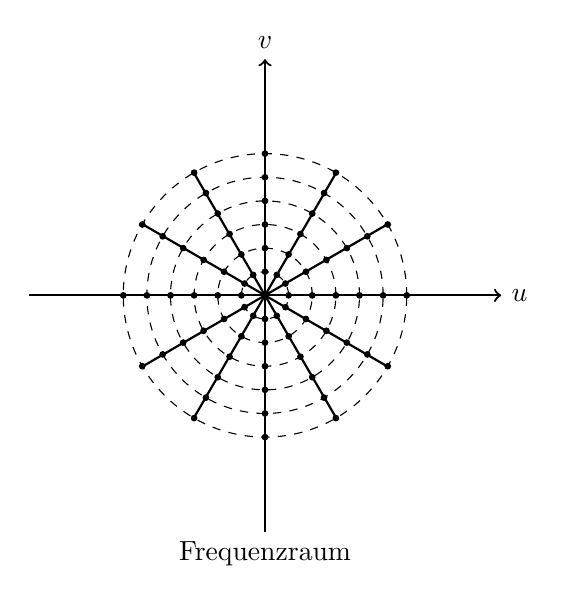
\begin{tikzpicture}[axis/.style={thick,->}]
    \draw[axis] (-3, 0) -- (3, 0) node [right] {$u$};
    \draw[axis] (0, -3) -- (0, 3) node[pos=0,below] {Frequenzraum} node [above] {$v$};

    % Kreise
    \draw[dashed] (0, 0) circle (3mm);
    \draw[dashed] (0, 0) circle (6mm);
    \draw[dashed] (0, 0) circle (9mm);
    \draw[dashed] (0, 0) circle (12mm);
    \draw[dashed] (0, 0) circle (15mm);
    \draw[dashed] (0, 0) circle (18mm);

    % Linien
    \draw[thick] (-1.55, -0.9) -- (1.55, 0.9);
    \draw[thick] (-0.9, -1.55) -- (0.9, 1.55);
    \draw[thick] (0.9, -1.55) -- (-0.9, 1.55);
    \draw[thick] (1.55, -0.9) -- (-1.55, 0.9);

    % Punkte
    \foreach \w in {0,...,6}
        \draw[fill=black] (0, 0 + \w * 0.3) circle (1pt);
    \foreach \w in {0,...,6}
        \draw[fill=black] (0, 0 - \w * 0.3) circle (1pt);

    \foreach \w in {0,...,6}
        \draw[fill=black] (0 + \w * 0.3, 0) circle (1pt);
    \foreach \w in {0,...,6}
        \draw[fill=black] (0 - \w * 0.3, 0) circle (1pt);

    \foreach \w in {0,...,6}
        \draw[fill=black] (30:\w * 3mm) circle (1pt);
    \foreach \w in {0,...,6}
        \draw[fill=black] (60:\w * 3mm) circle (1pt);
    \foreach \w in {0,...,6}
        \draw[fill=black] (120:\w * 3mm) circle (1pt);
    \foreach \w in {0,...,6}
        \draw[fill=black] (150:\w * 3mm) circle (1pt);
    \foreach \w in {0,...,6}
        \draw[fill=black] (210:\w * 3mm) circle (1pt);
    \foreach \w in {0,...,6}
        \draw[fill=black] (240:\w * 3mm) circle (1pt);
    \foreach \w in {0,...,6}
        \draw[fill=black] (300:\w * 3mm) circle (1pt);
    \foreach \w in {0,...,6}
        \draw[fill=black] (330:\w * 3mm) circle (1pt);
\end{tikzpicture}
\end{document}
